\chapter{Implementação}

Neste Capítulo estão relacionadas as atualizações e melhorias feitas no aplicativo ColetaCacau para uso de RFID, bem como a especificação e arquitetura do sistema para atender esta nova demanda.

\section{Tecnologias Utilizadas}
O React Native foi escolhido para permitir o desenvolvimento multiplataforma, otimizando o tempo e os custos ao oferecer uma interface responsiva tanto para \textit{Android} quanto \textit{iOS} \cite{Erz2020IoTBM}. Para garantir o armazenamento local das informações coletadas no campo, mesmo sem conectividade, foi implementado o RealmDB, que sincroniza os dados assim que a internet se torna disponível \cite{Appiah2024PlanteSaineAA}.

O gerenciamento de estado global do aplicativo foi facilitado pelo Redux, garantindo consistência nos dados e fluidez na navegação \cite{Akter2023AgroBasedMA}. Além disso, o \textit{Sentry} foi integrado para monitoramento de erros em tempo real, promovendo estabilidade e confiabilidade do sistema, mesmo em cenários críticos de operação em campo.

\section{Leitor RFID Utilizado}
O leitor RFID utilizado no ColetaCacau é um modelo \textit{USB Contactless}, originalmente projetado para atuar como dispositivo de teclado \textit{HID} (\textit{Human Interface Device}), que facilita a integração e operação \textit{plug-and-play} com diversos sistemas, dispensando a necessidade de instalação de drivers complexos. Esse leitor, operando em frequência de 125KHz, possui uma antena de transceptor embutida, garantindo a captação de sinais mesmo sem linha direta de visão, característica essencial para o ambiente agrícola.

Compatível com padrões de cartões \textit{ISO14443A}, \textit{NTAG203}, \textit{Ultraleve}, \textit{Classic 1k (s50)} e \textit{Classic 4k (s70)}, o leitor oferece suporte a uma variedade de tags, possibilitando flexibilidade na escolha dos dispositivos de marcação. Ele é capaz de ler apenas o UID (Identificador Único) das tags, com saídas de 4 a 7 \textit{bytes} do número de série do chip, fornecendo informações essenciais para identificar cada árvore no sistema sem expor dados adicionais.

Alimentado via interface USB com tensão DC de 5V, o leitor facilita a implementação no campo, utilizando a alimentação diretamente do dispositivo ao qual está conectado, seja um dispositivo móvel ou um computador. Seu tempo de leitura de cartões é extremamente rápido, geralmente inferior a 100ms, o que permite que o coletor obtenha feedback instantâneo durante a coleta. Além disso, possui indicadores LED duplos, que informam o estado da leitura e facilitam o uso em condições de luz variável, frequentes em ambientes externos. Essas especificações do leitor tornam-no uma escolha eficiente e acessível para a implementação no ColetaCacau, contribuindo para a redução dos custos operacionais e proporcionando uma experiência de uso prática e robusta no campo.

Para os testes realizados tanto em campo quanto localmente, foram utilizados dois modelos de leitores RFID, ambos dentro das especificações descritas anteriormente. Esses modelos são ilustrados na Figura \ref{fig:RfidModels}, que apresenta as versões dos leitores \textit{USB} e \textit{USB-C}. 

\begin{figure}[H]
    \centering
    \begin{minipage}[b]{0.45\textwidth}
        \centering
        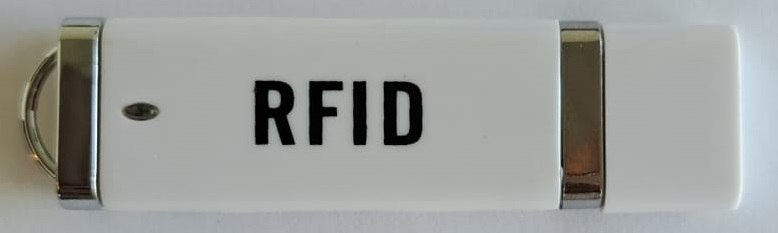
\includegraphics[width=\textwidth]{images/rfid/reader-01.jpg}
        \caption*{Leitor RFID - modelo USB.}
    \end{minipage}
    \hspace{5pt}
    \begin{minipage}[b]{0.35\textwidth}
        \centering
        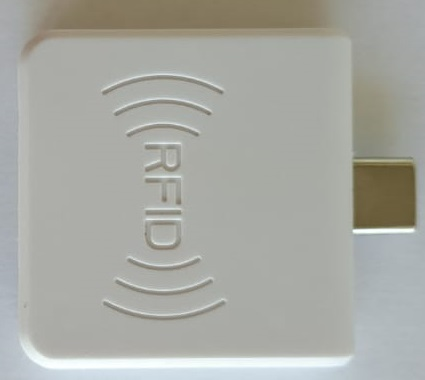
\includegraphics[width=\textwidth]{images/rfid/reader-02.jpg}
        \caption*{Leitor RFID - modelo USB-C.}
    \end{minipage}
    \hspace{5pt}
    
    \caption{Modelos de leitores RFID utilizados nos testes.}
    \label{fig:RfidModels}
\end{figure}

No aplicativo ColetaCacau, o leitor RFID é utilizado para captar as tags vinculadas a cada árvore no campo. Quando o coletor se aproxima da árvore equipada com a tag RFID, o sistema identifica automaticamente a tag lida e direciona o coletor para a árvore correspondente, integrando-se ao banco de dados \textit{RealmDB} para consultar e exibir as informações da árvore na interface. Esse processo automatizado elimina a necessidade de identificação manual, reduzindo significativamente o risco de erros operacionais e otimizando o tempo do coletor.

A programação do aplicativo permite que os sinais do leitor RFID sejam imediatamente associados ao banco de dados \textit{offline}, promovendo a sincronização entre a leitura em campo e o banco de dados do sistema, garantindo que o coletor visualize apenas a árvore correta sem qualquer ação manual adicional.

A Figura \ref{fig:RfidReader} ilustra o leitor RFID utilizado no ColetaCacau, destacando tanto o estado normal quanto o estado ativo durante a leitura de uma tag RFID. Essa visualização evidencia os indicadores LED duplos que fornecem uma resposta visual ao usuário, simplificando a operação em ambientes de campo e melhorando a eficiência do processo de coleta de dados.

\begin{figure}[H]
    \centering
    \begin{minipage}[b]{0.45\textwidth}
        \centering
        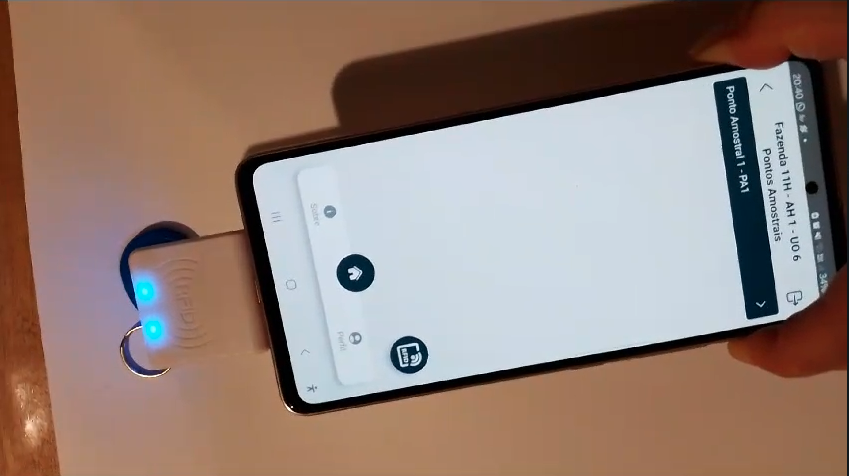
\includegraphics[width=\textwidth]{images/rfid/rfid-active.png}
        \caption*{(a) Estado Normal.}
    \end{minipage}
    \hspace{5pt}
    \begin{minipage}[b]{0.45\textwidth}
        \centering
        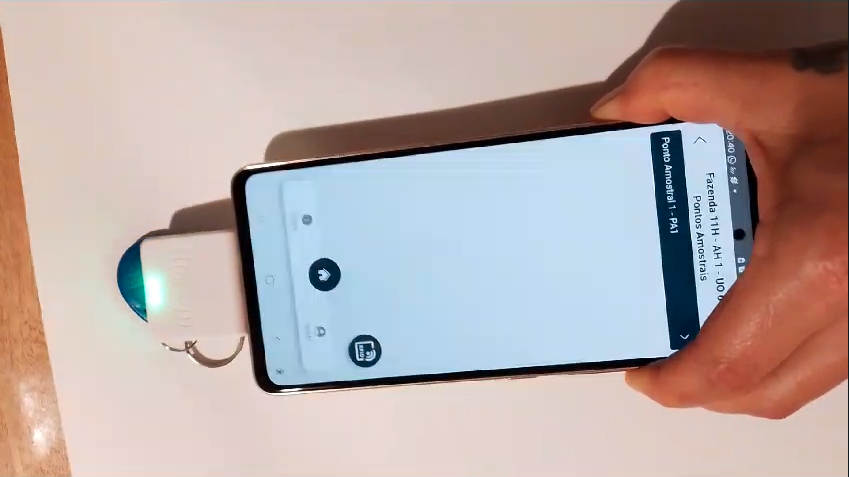
\includegraphics[width=\textwidth]{images/rfid/rfid-reading.png}
        \caption*{(b) Estado de Leitura.}
    \end{minipage}
    \hspace{5pt}
    
    \caption{Leitor RFID em dois estados: (a) Normal e (b) Ativo durante a leitura de uma tag.}
    \label{fig:RfidReader}
\end{figure}

\section{Tags RFID e Vinculação às Árvores}
No ColetaCacau, foram utilizadas tags RFID passivas de baixa frequência (12KHz) devido ao baixo custo de implementação e à durabilidade necessária para uso em campo, resistindo a intempéries e condições adversas. Cada tag RFID possui um identificador único constituído por uma sequência de 10 números aleatórios, garantindo a individualidade de cada árvore. Durante o cadastro, as tags são vinculadas a árvores específicas no sistema de gestão PlataformaCacau, permitindo que o aplicativo reconheça cada árvore automaticamente por meio da leitura da tag.

Cada código RFID é também vinculado à propriedade agrícola à qual a árvore pertence, assegurando que a integridade do banco de dados seja mantida e evitando duplicidades em diferentes propriedades. Essa organização fortalece o controle das informações, permitindo que as coletas subsequentes sejam precisas e garantindo que os coletores retornem sempre às mesmas árvores monitoradas.

A escolha por leitores e tags de baixa frequência reflete a necessidade de acessibilidade e sustentabilidade para uso em escala agrícola. A frequência de 12KHz reduz a susceptibilidade a interferências em campo, proporcionando uma leitura mais confiável, mesmo em ambientes adversos, e facilitando a implementação em várias propriedades sem a necessidade de elevados investimentos em infraestrutura.

Optou-se por não utilizar gravadores RFID de início, mantendo o foco na simplicidade e eficiência do sistema. Gravadores, que permitem a programação de tags, aumentariam tanto o custo quanto a complexidade do sistema, além de requerer uma infraestrutura mais robusta para regravação de dados nas tags, conforme necessário. Como cada árvore de uma propriedade é identificada unicamente.

Foi adotada, nesta fase do projeto, a estratégia de adquirir as tags gravadas de fábrica, por questões de custos e simplificação do processo. O fornecedor garante que a identificação é única, mas caso uma tag já cadastrada seja escaneada, o sistema alerta o usuário sobre a duplicidade, prevenindo inconsistências nos registros e mantendo a integridade dos dados coletados. O custo de cada tag já gravada ficou em torno de R\$2,00. O leitor de RFID entre R\$120,00 e R\$150,00.

Na Figura \ref{fig:RfidTags01} estão as primeiras tags RFID cadastradas e vinculadas no sistema, destacando a organização inicial e a vinculação prática com as árvores de cacau. Já a Figura \ref{fig:RfidTags02} exibe um conjunto adicional de tags RFID, mostrando a ampliação da aplicação do sistema para maior cobertura e controle no monitoramento.

\begin{figure}[H]
    \centering
    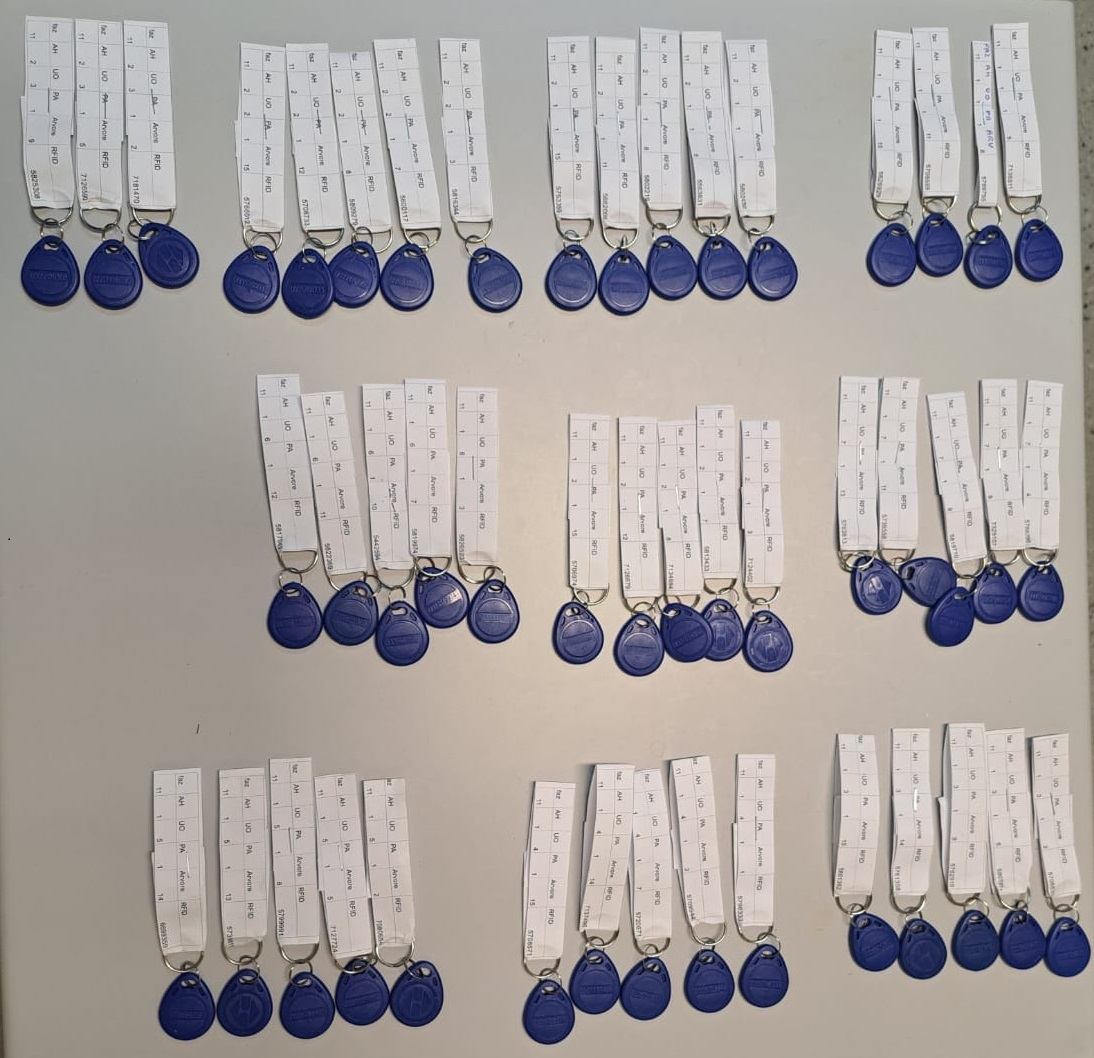
\includegraphics[width=0.6\textwidth]{images/rfid/rfid-tags-01.jpeg}
    \caption{Primeiras tags cadastradas e vinculadas (48 tags).}
    Autora: Marta M. Dornelles, 2024.
    \label{fig:RfidTags01}
\end{figure}

\begin{figure}[H]
    \centering
    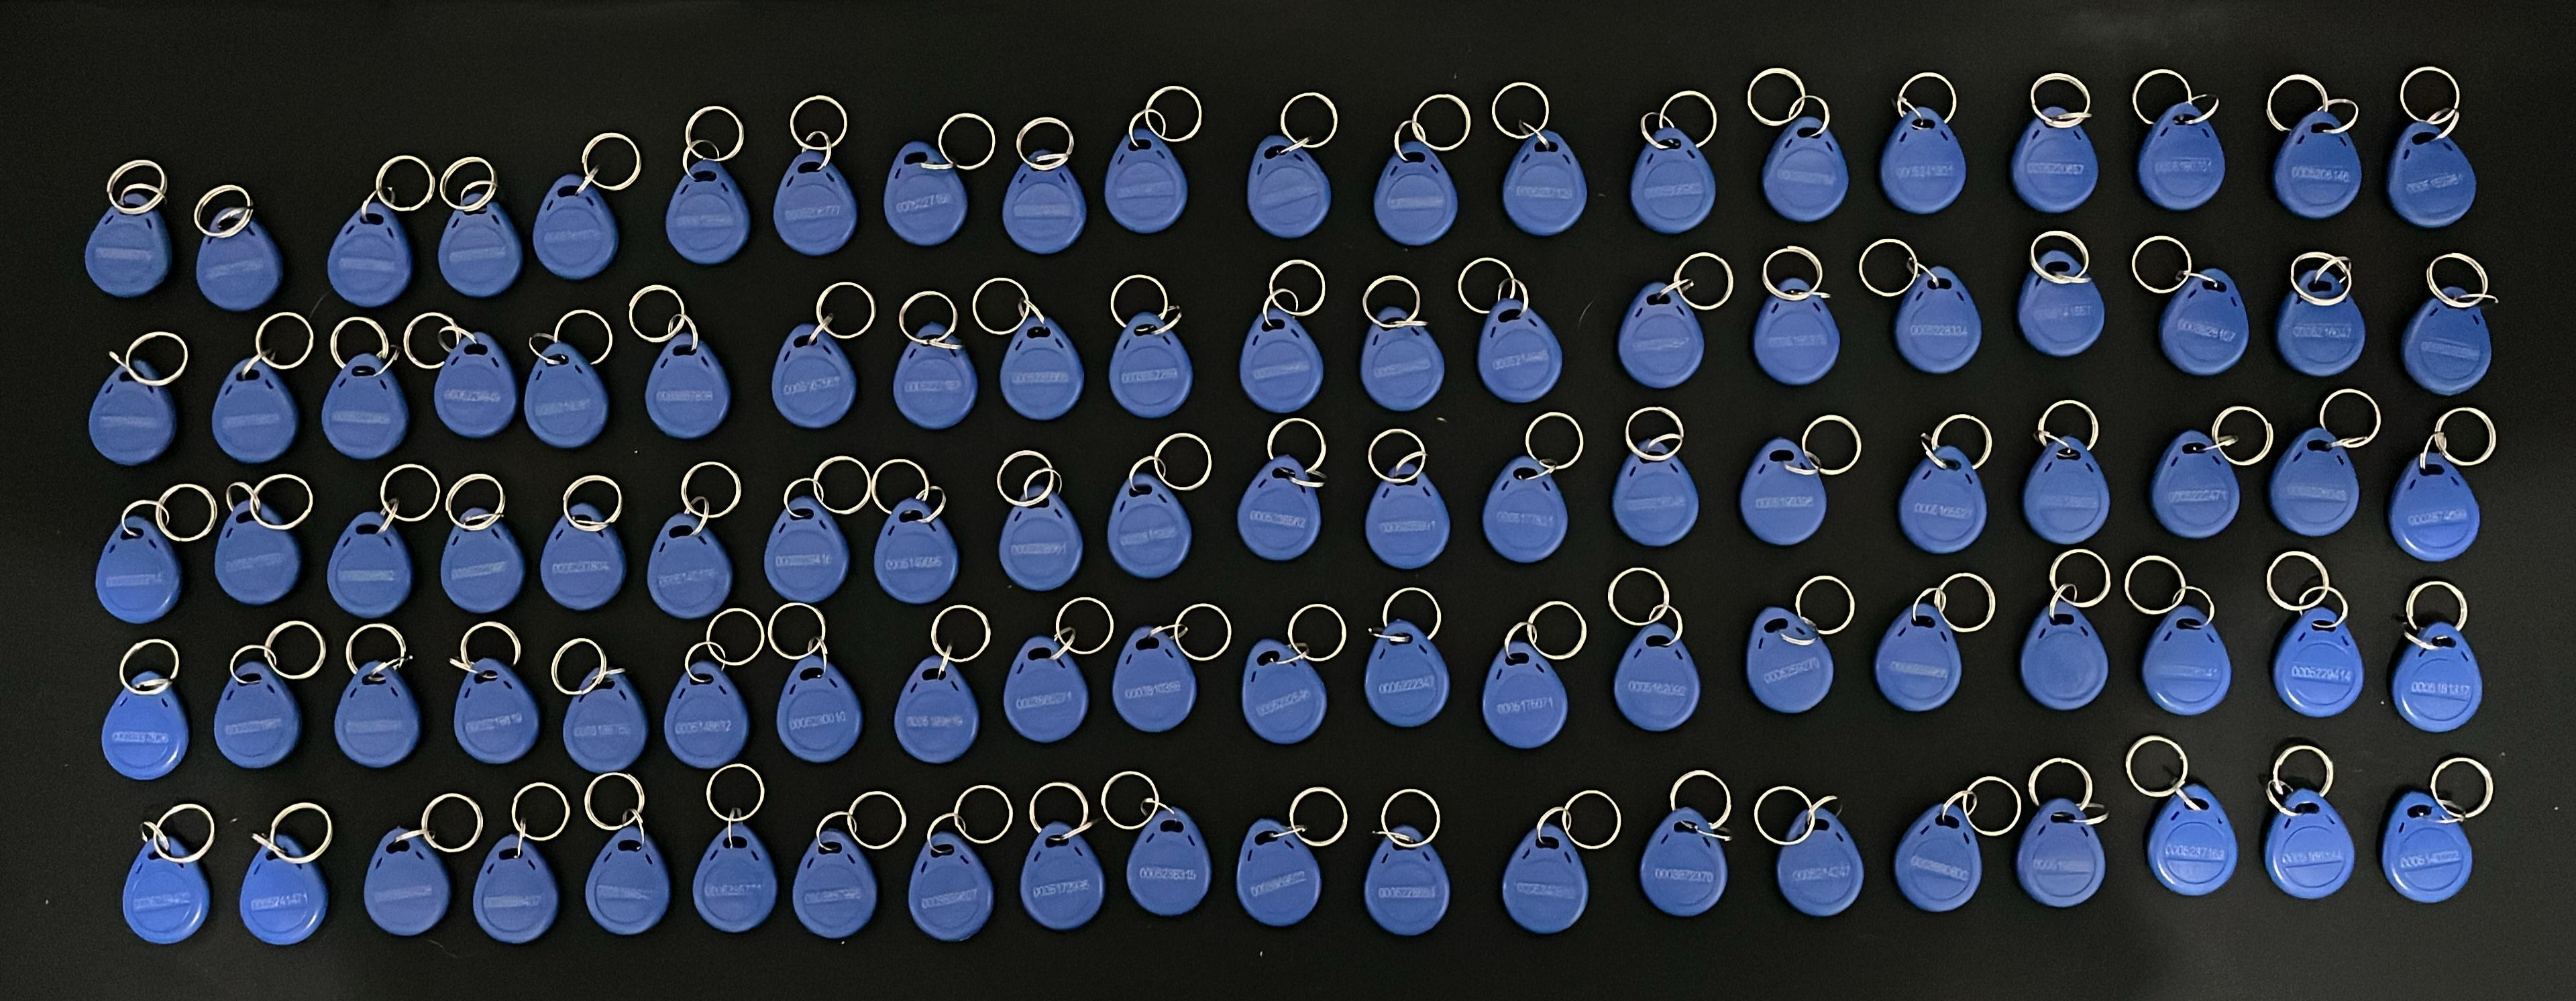
\includegraphics[width=0.8\textwidth]{images/rfid/rfid-tags-02.jpeg}
    \caption{Tags vinculadas posteriormente (92 tags).}
    Autor: Adriel F. da S. Oliveira, 2024.
    \label{fig:RfidTags02}
\end{figure}

Na Figura \ref{fig:RfidTag}, é apresentada uma visão detalhada da tag RFID utilizada, destacando o material e o código de 10 dígitos impresso na própria tag. Este código identifica exclusivamente cada árvore associada a uma propriedade no sistema ColetaCacau.

\begin{figure}[H]
    \centering
    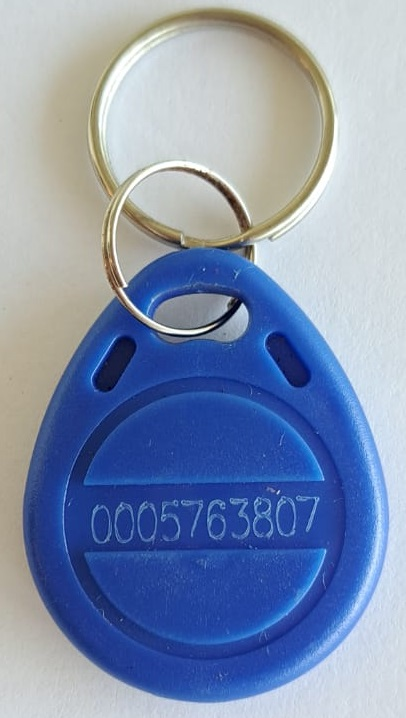
\includegraphics[width=0.4\textwidth]{images/rfid/tag.jpg}
    \caption{Tag RFID utilizada no ColetaCacau, com código impresso no material da tag.}
    \label{fig:RfidTag}
\end{figure}

\section{Módulo RFID Implementado}
O módulo RFID foi implementado com o objetivo de automatizar a identificação das árvores de cacau, melhorando a precisão e eficiência na coleta de dados em campo. Esse módulo é composto por uma integração entre o aplicativo móvel desenvolvido em React Native e um módulo nativo em Android, que gerencia a comunicação com o leitor RFID.

No React Native, o módulo de leitura de RFID utiliza a biblioteca \textit{NativeModules} para se comunicar diretamente com o hardware de leitura via USB. O leitor RFID, uma vez conectado ao dispositivo móvel, começa a capturar automaticamente as tags RFID associadas às árvores. Quando o coletor se aproxima de uma árvore equipada com a tag RFID, o sistema identifica a árvore e direciona o usuário para a tela correspondente no aplicativo, sem a necessidade de intervenção manual. Esse processo reduz significativamente os erros humanos, garantindo que os dados coletados sejam consistentes e mais precisos.

O \textit{layout} implementado oferece um campo de entrada para o código RFID e indicadores visuais claros sobre o status do leitor RFID (conectado ou desconectado). Quando uma tag RFID é lida com sucesso, o sistema fornece uma resposta visual imediata e direciona o coletor para o próximo passo no processo de coleta de dados.

A Figura \ref{fig:LayoutRfid} apresenta a tela do aplicativo, destacando a área de interação com a leitura das tags RFID.

\begin{figure}[H]
    \centering
    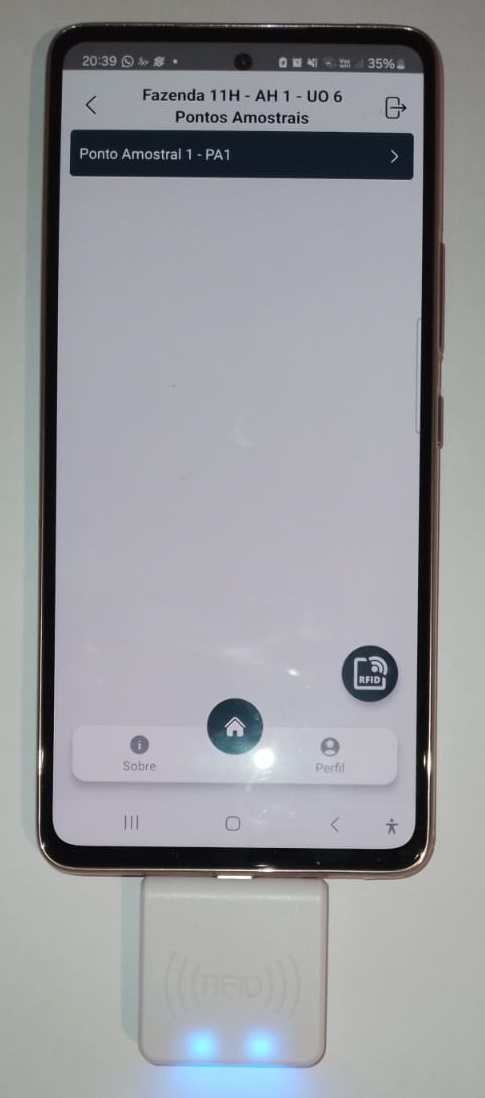
\includegraphics[width=0.35\textwidth]{images/rfid/phone.jpeg}
    \caption{Visulização completa do aplicativo com o leitor RFID}
    \label{fig:LayoutRfid}
\end{figure}

\section{Especificações}
O sistema ColetaCacau foi desenvolvido para otimizar a coleta de dados em campo, oferecendo funcionalidades avançadas que atendem às necessidades dos principais atores envolvidos no processo: os coletores e os gestores de fazendas. Abaixo, são detalhadas as especificações funcionais e não funcionais que guiaram o desenvolvimento do aplicativo.

Para garantir que as necessidades dos diferentes usuários sejam atendidas, o sistema ColetaCacau foi projetado com base em uma série de casos de uso. Os principais atores envolvidos são os coletores e os gestores de fazendas. Os coletores utilizam o aplicativo para registrar dados sobre as árvores e as áreas homogêneas, enquanto os gestores analisam esses dados para gerar relatórios de produtividade e acompanhar o progresso da safra. Na Figura \ref{fig:UseCasesDiagram} está a ilustração do diagrama de casos de uso com as principais interações desses atores com o sistema, detalhando as ações realizadas durante o processo de coleta de dados e análise.

\begin{figure}[H]
    \centering
    \frame{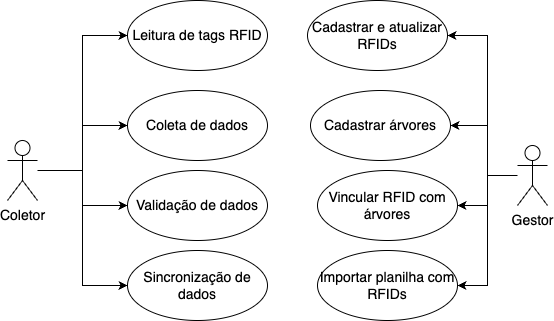
\includegraphics[scale=0.6]{images/diagrams/uc-diagram.png}}
    \caption{Diagrama de Casos de Uso.}
    \label{fig:UseCasesDiagram}
\end{figure}

\subsection{Requisitos Funcionais}
Os requisitos funcionais descrevem as funcionalidades que o sistema deve oferecer para atender às necessidades do usuário. No Quadro \ref{Tab:FunctionalReqs} a seguir estão descritos os requisitos funcionais (RF) atendidos pelo aplicativo.

\begin{quadro}[!htb]
    \centering
    \footnotesize
    \caption{Requisitos funcionais (RF).}
    \begin{tabular}{|c|p{4cm}|p{8cm}|}
        \hline
        \textbf{Identificação} & \centering\textbf{Nome} & \textbf{Descrição} \\
        \hline
        RF01          & Identificação Automática de Árvores         & O aplicativo deve ler as tags RFID das árvores e encaminhar o coletor automaticamente para tela da árvore respectiva.\\ \hline
        
        RF02          & Coleta \textit{Offline}          & O aplicativo deve funcionar completamente \textit{offline}, permitindo que os coletores registrem dados de campo sem necessidade de conexão com a internet. Os dados serão sincronizados posteriormente, quando a conexão estiver disponível. \\ \hline
        
        RF03          & Gerenciamento de Dados       &  O aplicativo deve possibilitar o armazenamento, edição e visualização dos dados coletados, permitindo que os usuários verifiquem informações sobre as árvores monitoradas e o progresso da safra.\\ \hline
        
        RF04          & Validação dos dados da coleta & O sistema deve incluir mecanismos para validar os dados inseridos pelos coletores, evitando a entrada de informações inconsistentes ou incompletas. Isso pode ser feito através de validações automáticas, que verificam se todos os campos obrigatórios foram preenchidos corretamente antes de permitir que os dados sejam salvos ou sincronizados com o servidor.\\ \hline
        
        RF05          & Cadastro de RFIDs & O sistema deve permitir que o gestor cadastre as tags RFID no banco de dados.\\ \hline
        
        RF06          & Vinculação de RFID com árvores & O sistema deve permitir que o gestor vincule cada RFID a uma árvore específica.\\ \hline

    \end{tabular}
    \label{Tab:FunctionalReqs}
    \fonte{o autor, 2024.}
\end{quadro}
\newpage

\subsection{Requisitos Não Funcionais}
Os requisitos não funcionais tratam das restrições e qualidades que o sistema deve atender. O Quadro \ref{Tab:NonFunctionalReqs} descreve os requisitos relacionados a certas restrições do sistema e aspectos de qualidade tanto do sistema quanto ao processo de desenvolvimento. 

\begin{quadro}[H]
	\centering
		\footnotesize
	\caption{Requisitos não funcionais (RNF).}
	\begin{tabular}{|c|p{8cm}|c|}
		\hline
		\textbf{Identificação} & \centering\textbf{Descrição} & \textbf{Classificação}\\
		\hline
		RNF01 & O aplicativo deve ser rápido e responsivo, mesmo em dispositivos móveis com capacidade limitada, garantindo uma experiência fluida ao usuário.   & Requisito de desempenho  \\ \hline
		
		RNF02 & Todas as informações coletadas devem ser armazenadas de forma segura e localmente, seguindo os padrões da Lei Geral de Proteção de Dados (LGPD).    & Requisito de segurança dos dados  \\ \hline
		
		RNF03 & O aplicativo deve ser compatível com as versões mais recentes dos sistemas operacionais Android e iOS. & Requisito de compatibilidade \\ \hline
		
		RNF04 & O aplicativo deve ser desenvolvido utilizando a o padrão de arquitetura MVVM (Movel, View, View-Model). & Requisito de implementação \\ \hline
		
		RNF05 & O \textit{design} do aplicativo deve ser simples e intuitivo, permitindo que os coletores, mesmo sem familiaridade com tecnologia, consigam utilizá-lo sem dificuldades. & Requisito de usabilidade \\ \hline
        
            RNF06 & O sistema deverá ser executado do Android 5.0 até o Android 14.  & Requisito de hardware \\ \hline

            RNF07 & O aplicativo deve ser capaz de realizar a leitura de tags no tempo limite de 1 segundo.  & Requisito de desempenho \\ \hline
	\end{tabular}
	\fonte{o autor, 2024.}
    \label{Tab:NonFunctionalReqs}
\end{quadro}

\section{Arquitetura do Sistema}
A arquitetura do sistema ColetaCacau, representada no diagrama C4 da Figura \ref{fig:C4Diagram}, foi cuidadosamente projetada para atender às necessidades de coleta de dados em ambientes rurais, garantindo eficiência e resiliência mesmo em condições de conectividade limitada. O sistema é composto por três camadas principais: interface, lógica de aplicação e dados. Além disso, inclui a PlataformaCacau, desenvolvida em \textit{Vue.js}, e uma API robusta construída em \textit{Laravel} para gerenciar e centralizar os dados coletados em campo.

\begin{figure}[H]
    \centering
    \frame{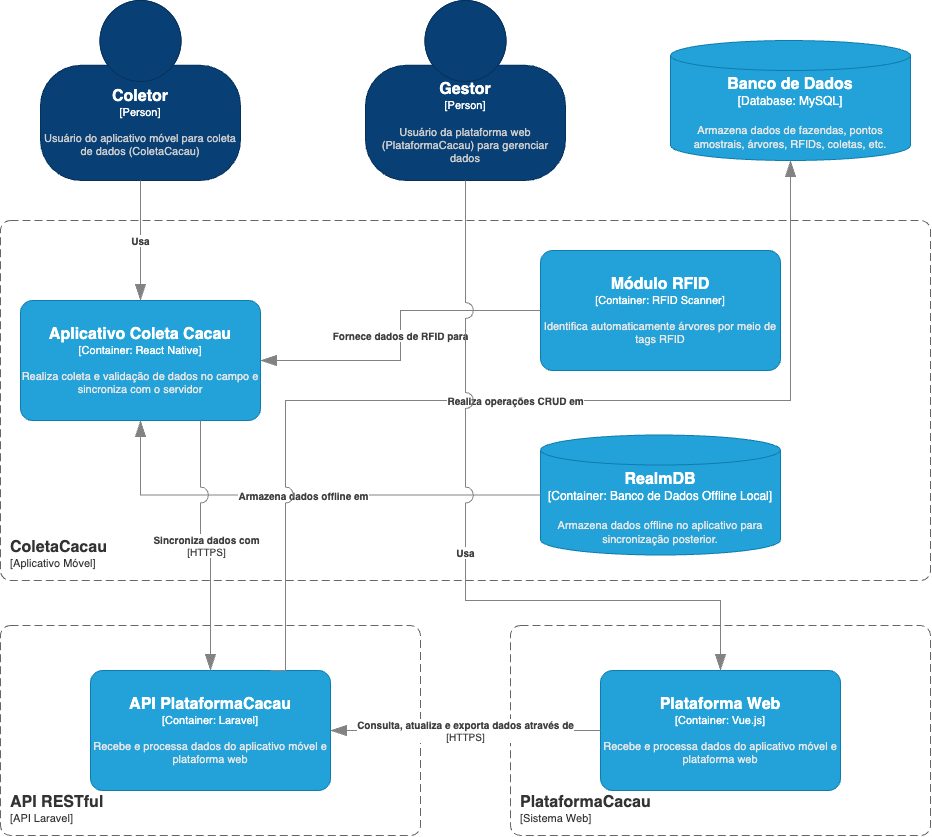
\includegraphics[width=\textwidth]{images/diagrams/c4-diagram.png}}
    \caption{Arquitetura do sistema ColetaCacau.}
    \fonte{o autor, 2024.}
    \label{fig:C4Diagram}
\end{figure}

A Camada de Interface (\textit{Front-End}) abrange duas plataformas: o aplicativo móvel, desenvolvido em \textit{React Native}, e a PlataformaCacau, uma interface web intuitiva e responsiva desenvolvida em \textit{Vue.js}. Enquanto o aplicativo é utilizado pelos coletores no campo para leitura de tags RFID e coleta de dados \textit{offline}, a PlataformaCacau é utilizada por gestores para o gerenciamento de propriedades, análise de dados e visualização de informações sincronizadas.

A Camada de Lógica de Aplicação gerencia o fluxo de informações entre a interface (móvel e web) e a API do \textit{back-end}. Essa camada inclui funcionalidades como leitura de tags RFID, sincronização \textit{offline}-\textit{online} e orquestração de dados coletados. A integração do \textit{Redux} no aplicativo assegura a consistência do estado global, enquanto a API, desenvolvida em \textit{Laravel}, proporciona uma comunicação segura e eficiente entre o \textit{front-end} e a base de dados centralizada.

A Camada de Dados (\textit{Back-End}) utiliza o \textit{RealmDB} no aplicativo móvel para armazenamento \textit{offline}, garantindo a operação em áreas remotas. A API \textit{Laravel} centraliza os dados sincronizados em um banco de dados relacional, permitindo análises avançadas e backup seguro. Assim, informações coletadas no campo pelo aplicativo são disponibilizadas para gestores na PlataformaCacau, promovendo uma visão holística e detalhada das operações.

\section{Fluxo de Coleta e Operação}
O fluxo operacional do aplicativo ColetaCacau com RFID envolve as seguintes etapas:

\begin{enumerate}
    \item \textbf{Cadastro de Árvores:} O usuário cadastra a fazenda e as árvores que serão monitoradas. Cada árvore recebe uma tag RFID, que será associada ao seu identificador no sistema web. Cada tag é única para a fazenda em que esta sendo realizada a vinculação.

    \item \textbf{Cadastro de RFID:} O usuário cadastra RFIDs com um código de até 10 dígitos númericos.

    \item \textbf{Leitura de Tags:} Ao chegar no campo, o coletor utiliza o aplicativo para ler as tags RFID das árvores. O aplicativo identifica automaticamente a árvore e exibe as informações de coleta associadas a ela.

    \item \textbf{Coleta de Dados:} O coletor preenche os dados de coleta, como o número de frutos, a condição da árvore e a qualidade da safra. Esses dados são armazenados localmente no RealmDB até que uma conexão à internet esteja disponível para sincronização.

    \item \textbf{Sincronização de Dados:} Quando o coletor retorna a uma área com conectividade, os dados armazenados \textit{offline} são automaticamente sincronizados com o servidor central, utilizando uma API segura.
\end{enumerate}

